\documentclass{beamer}
\usepackage[utf8]{inputenc}
\usepackage{amsmath, pdfpages, pdflscape, lscape, color, listings, hyperref, amssymb,graphicx,textcomp,varioref,afterpage,subcaption, float,color} 


% \makeatletter
% \def\input@path{{/home/simen/Dropbox/phd/presentations/presentations/neuronify}}
% %or: \def\input@path{{/path/to/folder}{/path/to/other/folder}}
% \makeatother

\title{Neuronify: a new tool to create models of simple neural networks}
\author{Simen Tennøe,\newline Svenn-Arne Dragly,\newline Andreas V. Solbr\aa,\newline Milad H. Mobarhan}

\usetheme{cinpla3}


\begin{document}
\maketitle

\begin{frame}
  \frametitle{This lecture inroduces Neuronify, a new tool to create simple neural networks}

  \begin{tikzpicture}[remember picture,overlay]  
    \node [xshift=-3.5cm,yshift=1.5cm] at (current page.center)
          {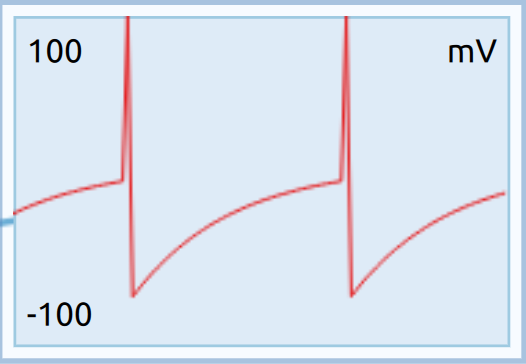
\includegraphics[width = 0.14\paperwidth ]{integrate.png}};
    \node [xshift=-2.cm,yshift=1.5cm, right] at (current page.center)
          { Integrate and Fire neurons};
  \end{tikzpicture}

  \begin{tikzpicture}[remember picture,overlay]  
    \node [xshift=-2cm,yshift=-.5cm] at (current page.center)
          {
\includegraphics[width = 0.12\paperwidth ]{logo.png}};
    \node [xshift=1cm,yshift=-.5cm, left] at (current page.center)
          { Neuronify };
  \end{tikzpicture}

  \begin{tikzpicture}[remember picture,overlay]  
    \node [xshift=-.5cm,yshift=-2.5cm] at (current page.center)
          {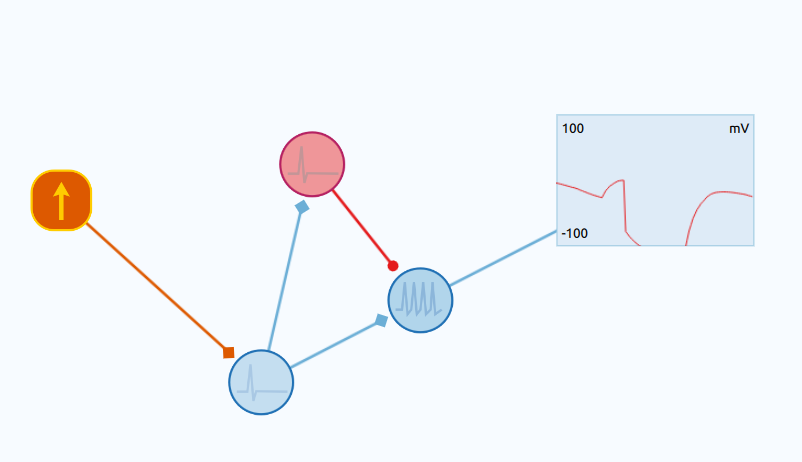
\includegraphics[width = 0.2\paperwidth ]{exercises.png}};
    \node [xshift=2.8cm,yshift=-2.5cm, left] at (current page.center)
          { Ecercises};
  \end{tikzpicture}

\end{frame}

\begin{frame}
\frametitle{The integrate and fire neuron is modeled as a simple RC circuit that is shortcircuted once a threshold is reached}
\begin{figure}
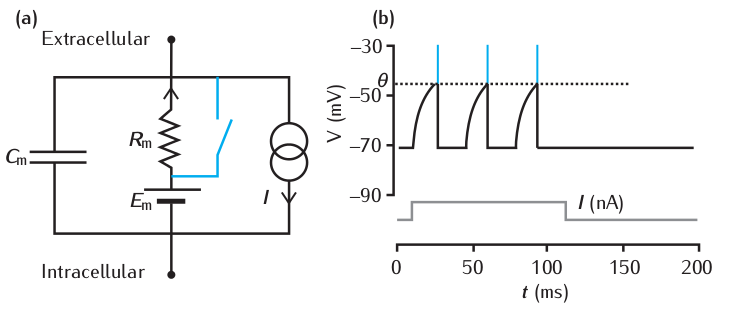
\includegraphics[width = \textwidth]{rc.png}
\end{figure}
\end{frame}

\begin{frame}
\frametitle{The integrate and fire neuron model is one of the simplest neuron models that exist and are therefore good for network models}
\end{frame}

\begin{frame}
\frametitle{Neuronify }
\end{frame}

\end{document}
